\documentclass[11pt,a4paper]{report}

\usepackage[polish]{babel}
\usepackage[utf8x]{inputenc}
\usepackage{polski}
%\usepackage[T1]{fontenc}
\frenchspacing
\usepackage{indentfirst}
\usepackage{amsthm}
\usepackage{amsmath}
\usepackage{algorithmic}
\usepackage{algorithm}
\usepackage{program}
\usepackage{programs}
\usepackage{array}
\usepackage{multirow}
\usepackage{graphicx}
\usepackage{listings}
\usepackage{listing}
\usepackage{float}
\pagenumbering{arabic}

\graphicspath{{img/}}

\begin{document}
\tableofcontents
\chapter{Macierze}
\section{Tworzenie macierzy na potrzeby algorytmów}
W algorytmach potrzebne są głównie 3 rodzaje macierzy i ich transpozycje. Macierze te są tworzone z danych zebranych z serwisu delicous:
\begin{itemize}
	\item $M_{UT}$ macierz ta zawiera w komórce $m_{n,m}$ informacje o ilości dokumentów dodanych przez użytkownika $u_n$ i opisanych tagiem $t_m$. Dane, z których zostaje utworzona ta macierz znajdują się w tabeli TAG\_USR. Tabela ta została wyliczona w czasie preprocessingu.
	\item $M_{TD}$ macierz ta zawiera w komórce $m_{n,m}$ informacje o ilości użytkowników którzy opisali tagiem $t_n$ dokument $d_m$. Źródłem danych dla taj macierzy jest tabela TAG\_DOC
	\item $M_{DU}$ analogicznie, ta macierz zawiera dane na temat ilości tagów. Informacje pobierane są z tabeli USERTAGDOC
\end{itemize}

Wykorzystywane są one w kolejnych iteracjach algorytmu Social PageRank. Przy algorytmie Adapted PageRank również są one używane pośrednio. Struktura na której operuje algorytm Adapted pagerank jest macierzą złozoną z macierzy $M_{UD} , M_{TD}, M_{UT}$ i ich transpozycji. Macierzy używana w algorytmie wygląda następująco:

\[
 G_f =
 \begin{pmatrix}
  0                     & M_{DU}       & M_{TD}^T \\
  M_{DU}^T  & 0                     & M_{UT}     \\
  M_{TD}       & M_{UT}^T   & 0 
 \end{pmatrix}
\]

Ważną cechą macierzy na których przeprowadzane są operacje jest to, że są to macierze rzadkie. Liczba niezerowych komórek w macierzy wynosi: 

\section{Operacje przeprowadzane na macierzach}
W każdej iteracji algorytmów główna operacją przeprowadzaną jest mnożenie wymienionych wcześniej macierzy przez wektor. Operacja ta jest przeprowadzana do czasu uzyskania zbieżności wartości wektora wynikowego.

Z powodu wielkości macierzy w aplikacji nie możemy wczytać bezpośrednio całych macierzy do pamięci i na nich operować. Dodatkowo używana biblioteka stawia ograniczenie na iloczyn kolumn i wierszy takie że: $ilosc\_kolumn * ilosc\_wierszy <= 2^{31}-1$.  Gdzie wartość $2^{31}-1$ jest to maksymalna liczba jaką można przypisać zmiennej typu integer w języku Java. 



\subsection*{Implementacja}

\begin{figure}[htb]
\centering
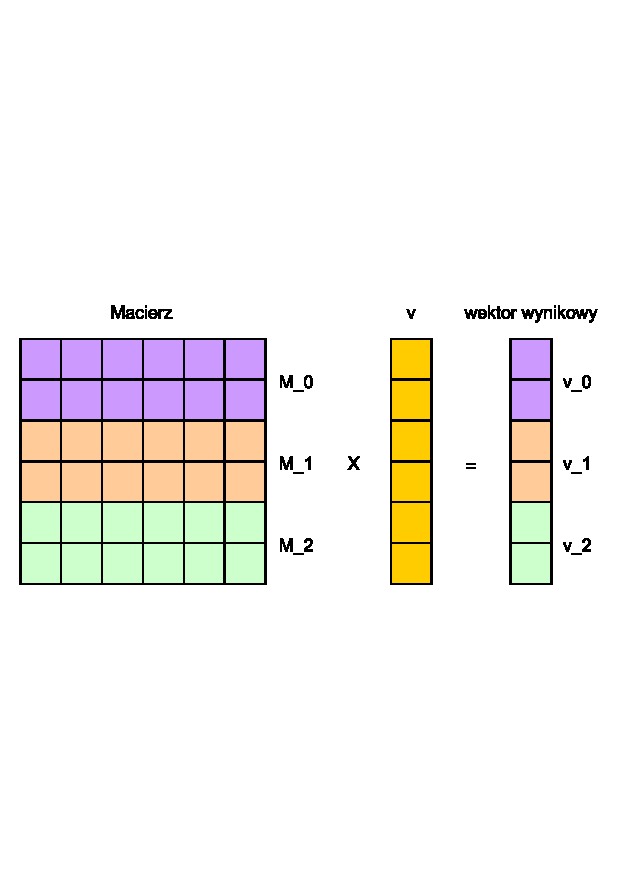
\includegraphics[width=1\textwidth, trim = 0mm 45mm 0mm 50mm, clip]{matrix_multiply.pdf}
\caption{Mnożenie macierzy przez wektor v}
\label{fig:matrix_mult_fig}
\end{figure}

Mnożenie macierzy odbywa się częściami. Bierzemy fragment macierzy: $M_{n}$ i mnożymy go przez wektor $v$. Wynikiem jest wektor $p_n$, który stanowi n-ty fragment wynikowego wektora. Powstałe fragmenty wektora łączymy razem, w odpowiedniej kolejności otrzymując w ten sposób w wektor wynikowy (\ref{fig:matrix_mult_fig})




\lstset{language=Python}
\begin{lstlisting}[frame=lines, caption={Mnożenie macierzy przez wektor v}, label={list:matrix_mult_fig}] ]
def matrix_multiply(v, matrix_source):
	v_return = empty_vector()  #wektor zwracany
	for matrix_part in matrix_source.get_part_matrixes():
		#mnozenie macierzy i wektora
		v_part = multiply(matrix_part, v) 
		# dokladamy wyliczony fragment wektora na koniec
		v_return.append(v_part)   
	return v_return 
\end{lstlisting}

Mnożenie odbywa się poprzez funkcje z biblioteki Colt. Biblioteka ta uwzględnia to, że macierz na której odbywają się operacje jest macierzą rzadką. Oszczędzana jest pamięć przez zapisywanie tylko niezerowych elementów. W czasie mnożenia przez wektor pomijane są wszystkie zerowe komórki, przez co sama operacja mnożenia jest krótka. Najwięcej czasu zajmuje samo tworzenie częściowych  macierzy i ładowanie plików zawierających kolejne fragmenty macierzy. 


\subsection{Metody przyśpieszenia obliczeń}

Opisana powyżej metoda nie mogłaby zostać wykorzystana w działającej. Przy tylko 1 milionie dokumentów czas wykonania algorytmu Social PageRank wynosi około 36 godzin. Prawdziwy system zawierałby zdecydowanie więcej danych. Poniżej opisanych jest kilka możliwych pomysłów na ulepszenie i przyśpieszenie działania aplikacji

\subsection*{Zmiana języka w którym została zaimplementowana aplikacja}
Maszyna wirtualna Javy nie jest bardzo wydajna jeśli chodzi o szybkość obliczeń, dodatkowo dochodzą ograniczenia związane np: z pamięcią. Możliwe jest również przepisanie tylko kluczowych dla obliczeń fragmentów, a następnie ich uruchamianie z aplikacji. 

\subsection*{Proste zrównoleglenie obliczeń}
Wykorzystując opisaną wcześniej metodę dzielenia macierzy na kawałki, możliwe jest podzielenie macierzy na różne procesory/maszyny. Każdy proces po zakończeniu obliczania swojej części zapisałby wynikowy wektor do np: bazy danych, w której następowałaby synchronizacja procesów. 

\subsection*{Obliczanie przy użyciu GPU/CUDA} 

Możliwe jest wykorzystanie GPU do wykonania obliczeń na macierzach. Obecne jednostki graficzne zawierają dodatkowe technologie wspomagające operacje na macierzach rzadkich. 

\subsection*{Wykorzystanie innych aplikacji}

Obliczanie kolejnych iteracji mogłoby również być przerzucone na zewnętrzną aplikacji np: MATLAB.



\end{document}
